% !TEX root = presentation.tex
\documentclass[aspectratio=169, 10pt]{beamer}

% ------------------------------------------------------------------------------
% Theme & Color Configuration (Ateneo Blue Palette)
% ------------------------------------------------------------------------------
\usetheme{Boadilla}
\usecolortheme{default}
\setbeamertemplate{navigation symbols}{}
\setbeamertemplate{blocks}[rounded][shadow=false]

% Custom Ateneo Color Definitions
\definecolor{AteneoBlue}{RGB}{0, 51, 102}        % #003366 Dark Navy
\definecolor{AteneoRoyal}{RGB}{0, 85, 165}       % #0055A5 Royal Blue
\definecolor{AteneoGold}{RGB}{217, 155, 0}       % #D99B00 Golden Accent
\definecolor{LightBlueBg}{RGB}{240, 244, 250}    % Soft slide block background
\definecolor{AlertRed}{RGB}{180, 40, 40}         % Safety / Warning accent
\definecolor{CardBorder}{RGB}{210, 220, 235}

% Apply Theme Colors
\setbeamercolor{structure}{fg=AteneoBlue}
\setbeamercolor{title}{fg=white, bg=AteneoBlue}
\setbeamercolor{frametitle}{fg=white, bg=AteneoBlue}
\setbeamercolor{author in head/foot}{fg=white, bg=AteneoBlue}
\setbeamercolor{title in head/foot}{fg=white, bg=AteneoRoyal}
\setbeamercolor{date in head/foot}{fg=white, bg=AteneoBlue}
\setbeamercolor{block title}{fg=white, bg=AteneoBlue}
\setbeamercolor{block body}{fg=black, bg=LightBlueBg}
\setbeamercolor{block title alerted}{fg=white, bg=AlertRed}
\setbeamercolor{block body alerted}{fg=black, bg=LightBlueBg}
\setbeamercolor{block title example}{fg=white, bg=AteneoRoyal}
\setbeamercolor{block body example}{fg=black, bg=LightBlueBg}
\setbeamercolor{item}{fg=AteneoRoyal}

% Custom Footline with Frame Numbering
\setbeamertemplate{footline}{
    \leavevmode%
    \hbox{%
    \begin{beamercolorbox}[wd=.333333\paperwidth,ht=2.25ex,dp=1ex,center]{author in head/foot}%
        \usebeamerfont{author in head/foot}Ateneo Computer Engineering Society
    \end{beamercolorbox}%
    \begin{beamercolorbox}[wd=.416666\paperwidth,ht=2.25ex,dp=1ex,center]{title in head/foot}%
        \usebeamerfont{title in head/foot}Electronics Workshop: Safety \& Components
    \end{beamercolorbox}%
    \begin{beamercolorbox}[wd=.25\paperwidth,ht=2.25ex,dp=1ex,right]{date in head/foot}%
        \usebeamerfont{date in head/foot}\insertframenumber{} / \inserttotalframenumber\hspace*{2ex}
    \end{beamercolorbox}}%
    \vskip0pt%
}

% ------------------------------------------------------------------------------
% Required Packages
% ------------------------------------------------------------------------------
\usepackage{booktabs}
\usepackage{amsmath, amssymb}
\usepackage{graphicx}
\usepackage{tabularx}
\usepackage{colortbl}
\usepackage{tikz}
\usetikzlibrary{arrows.meta, positioning, calc}

% ------------------------------------------------------------------------------
% Metadata
% ------------------------------------------------------------------------------
\title[Electronics Workshop Module]{\textbf{\Large Electronics Workshop Module}}
\subtitle{\large Laboratory Safety Protocols \& Electronic Components}
\author[Ateneo CoES]{\textbf{Ateneo Computer Engineering Society}}
\institute[ADNU]{Department of Computer Engineering}
\date{Academic Year 2026--2027}

% ------------------------------------------------------------------------------
% Document Content
% ------------------------------------------------------------------------------
\begin{document}

% !TEX root = ../presentation.tex

% ------------------------------------------------------------------------------
% Slide 1: Title Slide (Modeled after 5p-2627s1 Page 1)
% ------------------------------------------------------------------------------
\begin{frame}[plain]
    \titlepage
\end{frame}

\section{Introduction \& Objectives}

% ------------------------------------------------------------------------------
% Slide 2: Session Objectives
% ------------------------------------------------------------------------------
\begin{frame}{Session Objectives \& Scope}
    \begin{columns}[T]
        \begin{column}{0.48\textwidth}
            \textbf{What You Will Learn Today}
            \begin{itemize}
                \item \textbf{Laboratory Safety Compliance:} Recognize electrical physiological thresholds and shock hazards.
                \item \textbf{ESD Damage Prevention:} Static dissipation mechanisms and sensitive semiconductor handling.
                \item \textbf{Component Taxonomy:} Distinguish between passive and active electronic devices.
                \item \textbf{Packaging \& Pinouts:} Read polarity markings, transistor pin assignments, and DIP IC indexing.
            \end{itemize}
        \end{column}
        
        \begin{column}{0.48\textwidth}
            \textbf{Workshop Roadmap}
            \begin{itemize}
                \item \textbf{Part 1: Laboratory Safety Protocols}
                \begin{itemize}
                    \item Shock physics ($I = V/R_{\text{body}}$)
                    \item Physiological current thresholds
                    \item Workbench housekeeping \& ESD control
                \end{itemize}
                \item \textbf{Part 2: Electronic Components}
                \begin{itemize}
                    \item Passive components ($R$, $C$, $L$)
                    \item Active semiconductors (Diodes, LEDs, BJTs, ICs)
                    \item Essential circuit calculations
                \end{itemize}
            \end{itemize}
        \end{column}
    \end{columns}
\end{frame}

% !TEX root = ../presentation.tex

\section{Laboratory Safety Protocols}

\begin{frame}{The Physics of Electric Shock: Human Body as a Resistor}
    \begin{columns}[T]
        \begin{column}{0.52\textwidth}
            \textbf{Ohm's Law Applied to Human Tissue}
            $$I = \frac{V}{R_{\text{body}}}$$
            \begin{itemize}
                \item Voltage alone does not kill; \textbf{current magnitude ($I$)} and pathway dictate lethality.
                \item \textbf{Dry Skin:} $R \approx 10{,}000\,\Omega \text{ to } 100{,}000\,\Omega$.
                \item \textbf{Wet/Perspiring Skin:} $R$ plummets to $\le 1{,}000\,\Omega$.
                \item At $1{,}000\,\Omega$, a $50\,\text{V}$ line yields $50\,\text{mA}$---enough to trigger ventricular fibrillation.
            \end{itemize}
        \end{column}
        \begin{column}{0.44\textwidth}
            \textbf{The ``One-Hand Rule''}
            \begin{itemize}
                \item Keep \textbf{one hand in your pocket} or behind your back when probing live high-voltage test points.
                \item Prevents current from forming a cross-torso circuit through the heart (hand-to-hand pathway).
            \end{itemize}
        \end{column}
    \end{columns}
\end{frame}

\begin{frame}{Physiological Current Thresholds ($60\,\text{Hz}\text{ AC} / \text{DC}$)}
    \begin{table}[htbp]
        \small
        \centering
        \begin{tabularx}{\textwidth}{l p{4.2cm} X}
            \toprule
            \textbf{Current Level} & \textbf{Physiological Reaction} & \textbf{Clinical Hazard} \\
            \midrule
            $1\,\text{mA}$ & Perception Threshold & Faint tingling sensation; safe. \\
            $5\,\text{mA}$ & Maximum Harmless Current & Involuntary jerk; potential secondary trauma. \\
            $10\text{--}20\,\text{mA}$ & \textbf{``Let-Go'' Threshold} & Muscular paralysis; victim cannot release conductor. \\
            $20\text{--}50\,\text{mA}$ & Respiratory Arrest & Chest muscles contract; suffocation within minutes. \\
            $\ge 100\,\text{mA}$ & \textbf{Ventricular Fibrillation} & Heart quivers uncontrollably; fatal without immediate CPR/AED. \\
            \bottomrule
        \end{tabularx}
    \end{table}
\end{frame}

\begin{frame}{Workbench Safety, Housekeeping \& ESD Mitigation}
    \begin{columns}[T]
        \begin{column}{0.48\textwidth}
            \textbf{Personal Protective Equipment (PPE)}
            \begin{itemize}
                \item \textbf{ANSI Z87.1 Safety Glasses:} Mandatory during soldering and component lead clipping.
                \item \textbf{Zero Jewelry Policy:} Rings and metallic watchbands can short power rails, causing severe arc burns.
                \item \textbf{De-energized Prototyping:} Always disconnect power before inserting or pulling components.
            \end{itemize}
        \end{column}
        \begin{column}{0.48\textwidth}
            \textbf{Electrostatic Discharge (ESD) Standards}
            \begin{itemize}
                \item Human perception threshold for ESD is $\approx 3{,}000\,\text{V}$.
                \item CMOS/MOSFET gates suffer punch-through breakdown at $<100\,\text{V}$.
                \item \textbf{Wrist Straps:} Must include a \textbf{$1\,\text{M}\Omega$ safety resistor} to protect user from mains faults.
                \item Handle ICs by packaging body, never exposed pins.
            \end{itemize}
        \end{column}
    \end{columns}
\end{frame}

% !TEX root = ../presentation.tex

\begin{frame}{Component Taxonomy: Passive vs. Active Devices}
    \begin{columns}[T]
        \begin{column}{0.48\textwidth}
            \begin{block}{Passive Components}
                \textit{Cannot introduce net electrical energy or amplify.}
                \begin{itemize}
                    \item \textbf{Resistors ($R$):} Dissipate energy as heat ($P = I^2 R$).
                    \item \textbf{Capacitors ($C$):} Store energy in electric field ($E = \frac{1}{2}CV^2$).
                    \item \textbf{Inductors ($L$):} Store energy in magnetic field ($E = \frac{1}{2}LI^2$).
                \end{itemize}
            \end{block}
        \end{column}
        \begin{column}{0.48\textwidth}
            \begin{exampleblock}{Active Components}
                \textit{Require external DC bias; can amplify or switch.}
                \begin{itemize}
                    \item \textbf{Diodes / LEDs:} Unidirectional conduction ($V > V_F$).
                    \item \textbf{BJTs:} Current-controlled current source ($I_C = \beta I_B$).
                    \item \textbf{MOSFETs:} Voltage-controlled channel switching.
                    \item \textbf{ICs:} Monolithic integration of micro-circuits.
                \end{itemize}
            \end{exampleblock}
        \end{column}
    \end{columns}
\end{frame}

\begin{frame}{Resistors: Color Codes \& Power Ratings}
    \begin{columns}[c]
        \begin{column}{0.48\textwidth}
            \begin{block}{Function \& Sizing}
                \begin{itemize}
                    \item Current limitation and potential division ($V = IR$).
                    \item Physical size correlates with \textbf{thermal power dissipation}, not resistance value!
                    \item Standard lab: $1/4\,\text{W}$ carbon/metal film.
                    \item High power: $1\,\text{W}, 2\,\text{W}$, up to $5\,\text{W}$ ceramic block.
                \end{itemize}
            \end{block}
        \end{column}
        \begin{column}{0.48\textwidth}
            \centering
            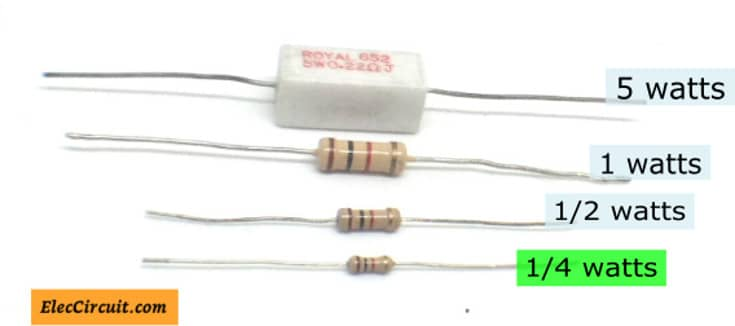
\includegraphics[width=\textwidth]{figures/fig_resistors.jpg}
        \end{column}
    \end{columns}
\end{frame}

\begin{frame}{Capacitors \& Inductors: Energy Storage}
    \begin{columns}[c]
        \begin{column}{0.48\textwidth}
            \begin{block}{Capacitor Types \& Polarity Danger}
                \begin{itemize}
                    \item \textbf{Ceramic (Non-polarized):} High frequency bypass ($10\,\text{pF}\text{--}100\,\text{nF}$).
                    \item \textbf{Electrolytic (Polarized):} High capacitance bulk filtering ($1\,\mu\text{F}\text{--}4700\,\mu\text{F}$).
                    \item \alert{Reverse polarity on electrolytics causes catastrophic electrolyte boiling and venting!}
                \end{itemize}
            \end{block}
        \end{column}
        \begin{column}{0.48\textwidth}
            \centering
            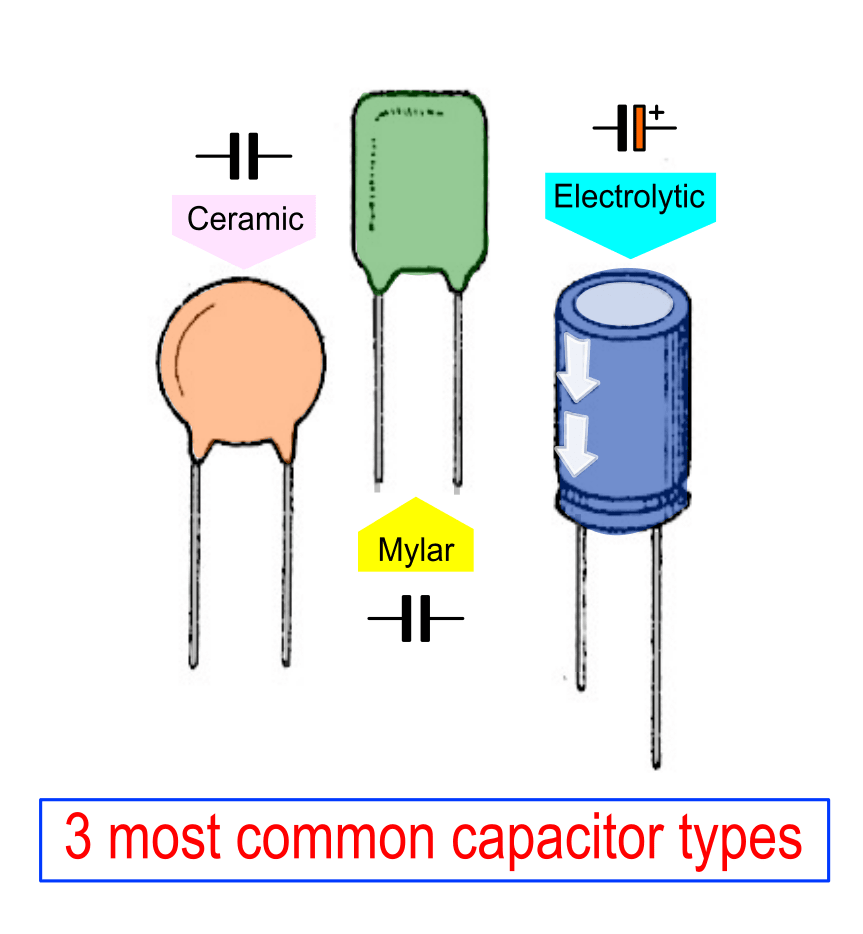
\includegraphics[width=0.9\textwidth]{figures/fig_capacitors.png}
        \end{column}
    \end{columns}
\end{frame}

\begin{frame}{Semiconductor Diodes \& Cathode Band Identification}
    \begin{columns}[c]
        \begin{column}{0.5\textwidth}
            \begin{block}{PN Junction Physics}
                \begin{itemize}
                    \item Acts as an electrical one-way check valve.
                    \item \textbf{Forward Bias ($V > V_F$):} Conduction initiates ($V_F \approx 0.7\,\text{V}$ for Silicon, $0.3\,\text{V}$ for Schottky).
                    \item \textbf{Reverse Bias:} Blocks current up to breakdown voltage $V_{BR}$.
                    \item \textbf{Physical Marking:} Silver/black band indicates the \textbf{Cathode ($K$)} terminal.
                \end{itemize}
            \end{block}
        \end{column}
        \begin{column}{0.46\textwidth}
            \centering
            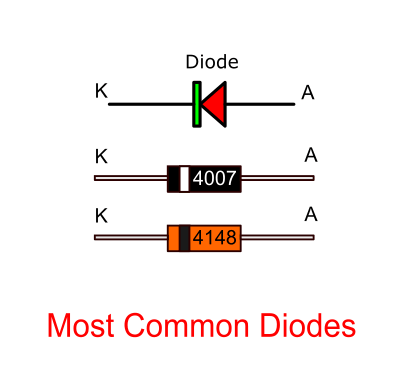
\includegraphics[width=\textwidth]{figures/fig_diodes.png}
        \end{column}
    \end{columns}
\end{frame}

\begin{frame}{Light Emitting Diodes (LEDs) \& Ballast Resistor Design}
    \begin{columns}[c]
        \begin{column}{0.52\textwidth}
            \begin{block}{Current-Limiting Formula}
                $$R = \frac{V_{CC} - V_F}{I_F}$$
                \textit{Example (5V DC Supply, Standard Red LED):}
                $$R = \frac{5.0\,\text{V} - 2.0\,\text{V}}{0.0091\,\text{A}} \approx 330\,\Omega$$
                \begin{itemize}
                    \item \textbf{Anode ($+$):} Longer lead.
                    \item \textbf{Cathode ($-$):} Shorter lead \& flat rim notch.
                \end{itemize}
            \end{block}
        \end{column}
        \begin{column}{0.44\textwidth}
            \centering
            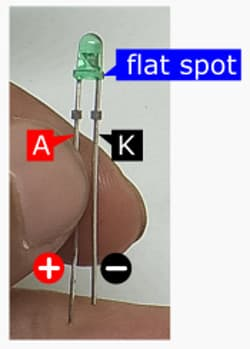
\includegraphics[height=2.4cm, keepaspectratio]{figures/fig_led_pinout.jpg}\\[0.2em]
            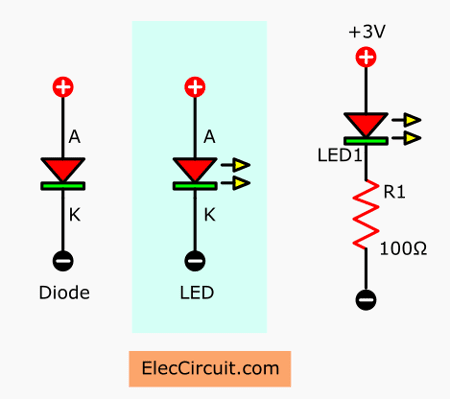
\includegraphics[height=1.8cm, keepaspectratio]{figures/fig_led_symbol.png}
        \end{column}
    \end{columns}
\end{frame}

\begin{frame}{Bipolar Junction Transistors (BJTs) \& Packaging}
    \begin{columns}[c]
        \begin{column}{0.5\textwidth}
            \begin{block}{Three-Terminal Switching}
                \begin{itemize}
                    \item Terminals: \textbf{Base (B)}, \textbf{Collector (C)}, \textbf{Emitter (E)}.
                    \item Small base current controls large collector current:
                    $$I_C = \beta I_B$$
                    \item \textbf{NPN:} Current flows Collector $\to$ Emitter when Base is positive.
                    \item Always verify pinouts (TO-92 packages vary across manufacturers: E-B-C vs. C-B-E).
                \end{itemize}
            \end{block}
        \end{column}
        \begin{column}{0.46\textwidth}
            \centering
            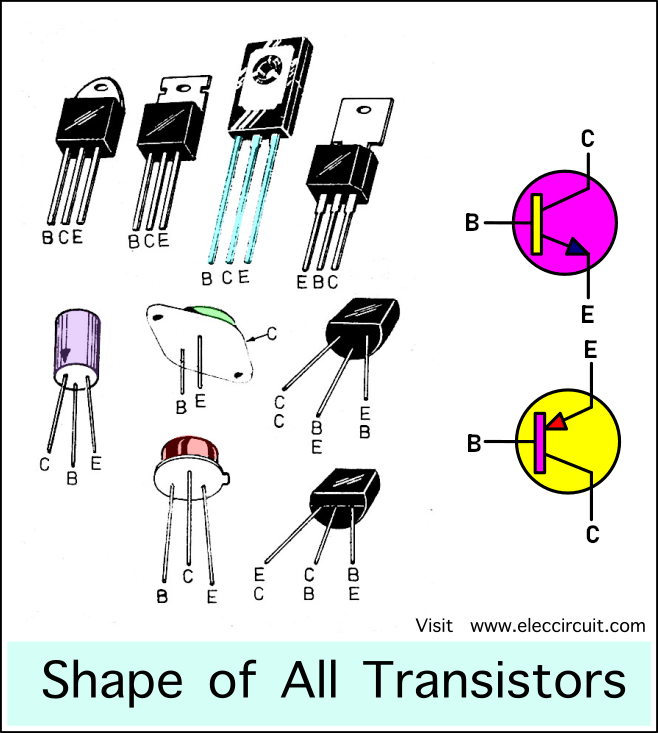
\includegraphics[width=\textwidth]{figures/fig_transistor_shapes.png}
        \end{column}
    \end{columns}
\end{frame}

\begin{frame}{Integrated Circuits (ICs) \& Dual In-Line Packaging (DIP)}
    \begin{columns}[c]
        \begin{column}{0.5\textwidth}
            \begin{block}{Pin 1 Orientation Convention}
                \begin{itemize}
                    \item \textbf{Alignment Notch:} Position the notch facing upward/leftward.
                    \item \textbf{Pin 1 Dot:} Directly adjacent to the notch.
                    \item \textbf{Counter-Clockwise Counting:} Numbering proceeds down the left column and continues up the right column.
                    \item Use IC extractors to avoid bending pins during removal.
                \end{itemize}
            \end{block}
        \end{column}
        \begin{column}{0.46\textwidth}
            \centering
            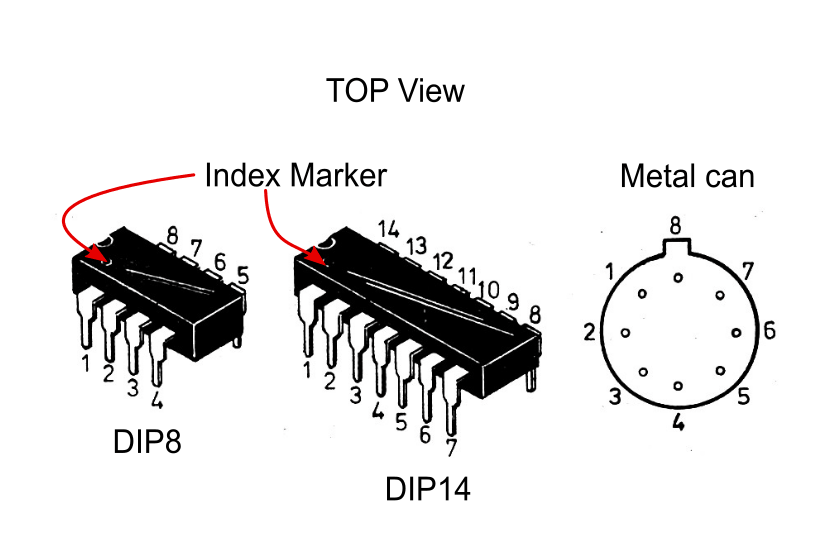
\includegraphics[width=\textwidth]{figures/fig_ic_packages.png}
        \end{column}
    \end{columns}
\end{frame}

% !TEX root = ../presentation.tex

\section{Summary \& Key Principles}

\begin{frame}{Summary of Key Principles}
    \begin{columns}[T]
        \begin{column}{0.48\textwidth}
            \textbf{Laboratory Safety Takeaways}
            \begin{itemize}
                \item Current ($I$) dictates biological shock hazard ($\ge 10\,\text{mA}$ freezes muscles).
                \item Practice the \textbf{One-Hand Rule} around energized circuits.
                \item Always wear \textbf{ANSI Z87.1 eye protection}.
                \item Use grounded wrist straps with \textbf{$1\,\text{M}\Omega$ safety resistor} for ESD mitigation.
            \end{itemize}
        \end{column}
        \begin{column}{0.48\textwidth}
            \textbf{Component Engineering Takeaways}
            \begin{itemize}
                \item Resistor physical volume reflects \textbf{power dissipation}, not ohms.
                \item Respect capacitor \textbf{polarity} to prevent explosive venting.
                \item Size series ballast resistors for LEDs using $R = (V_{CC} - V_F)/I_F$.
                \item Verify BJT pinouts (E-B-C) and locate IC \textbf{Pin 1} before powering.
            \end{itemize}
        \end{column}
    \end{columns}
\end{frame}

\begin{frame}[plain]
    \centering
    \vspace{2cm}
    {\Huge \textbf{Thank You!}}\\[1em]
    {\large \textbf{Questions \& Discussion}}\\[0.8em]
    \textbf{Ateneo Computer Engineering Society}\\[0.3em]
    \footnotesize Department of Computer Engineering $\cdot$ Academic Year 2026--2027
\end{frame}


\end{document}
